\section{Passo 12 — Planilha base, importação e encerramento}
\label{sec:passo12}

\subsection*{Objetivo}
Sair do aplicativo com os dados em formato aberto e com o estudo reprodutível por outra pessoa.

\begin{figure}[H]
\centering
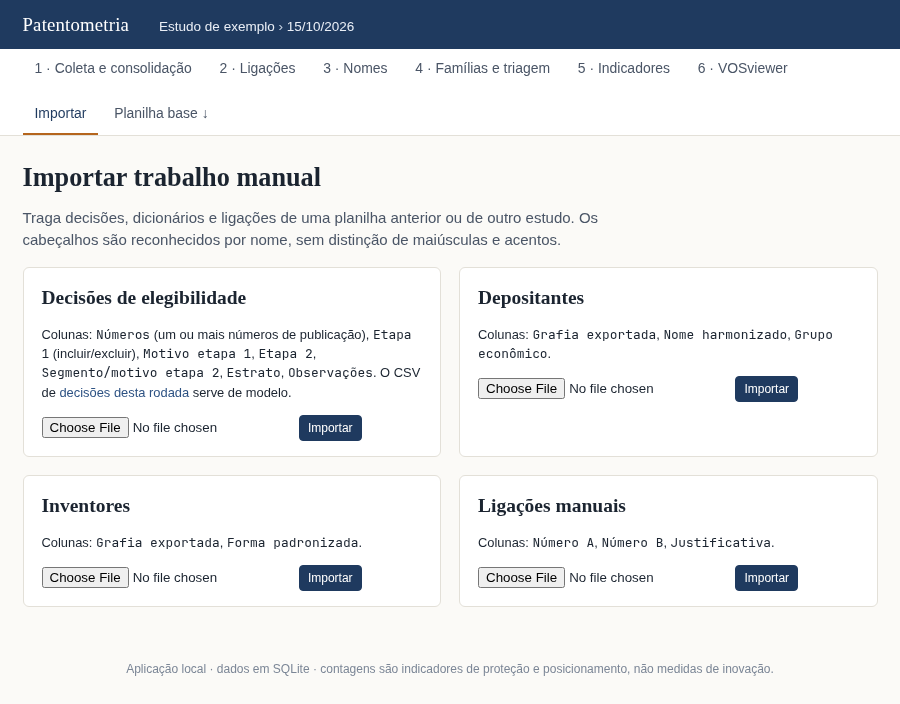
\includegraphics[width=0.9\linewidth]{img/14_importar.png}
\caption{Tela de importação: entrada de um estudo ou de uma planilha já preparada, com validação antes
de gravar.}
\label{fig:importar}
\end{figure}

\subsection*{O que fazer}
\begin{enumerate}
\item Clique em \textbf{Planilha base} para baixar o \campo{.xlsx} com famílias, decisões e indicadores.
\item Clique em \textbf{Decisões} para baixar o CSV com o rastro da triagem.
\item Em \textbf{Importar}, use o JSON exportado do estudo para reproduzi-lo em outra máquina.
\item Guarde a pasta de dados (banco e arquivos) junto do projeto.
\end{enumerate}

\subsection*{Como interpretar}
A planilha é a camada de auditoria: cada linha é uma família, com os campos consolidados e as decisões.
O CSV de decisões é o que permite reconstruir o PRISMA sem reabrir a aplicação.

O JSON de estudo contém a configuração, não os dados. Importar o JSON em outra instalação recria as
regras; os arquivos das bases precisam ser reenviados para reproduzir os números.

\begin{nota}[Checklist de encerramento]
\num{1)} PRISMA fechado e conferido; \num{2)} nenhuma família pendente nas etapas 1 e 2;
\num{3)} depositantes e inventores harmonizados; \num{4)} ligações aplicadas e reconsolidadas;
\num{5)} indicadores lidos com denominador e data; \num{6)} planilha e decisões exportadas;
\num{7)} backup da pasta de dados.
\end{nota}

\begin{alerta}[Erro comum]
Exportar a planilha antes da última reconsolidação. O arquivo nasce com os números do momento em que
foi gerado --- confira a data no cabeçalho.
\end{alerta}

\subsection*{Checkpoint}
\marcador\; Você consegue entregar a pasta do estudo com configuração, exportações, planilha, decisões e
backup, e outra pessoa consegue repetir a rodada seguindo este guia.
